\scanpage{24}
\mspage{\handwritten{15}}
$p$-linéaire\handwritten{\unsure{s|)|>}} opérant sur les $H^i(X,\underline{O}_X)$. Quitte à remplacer $k$ par une extension finie, on peut supposer que toutes les valeurs propres desdits frobenius sont égales à 0 ou 1. Soit $c$ la somme alternée \deleted{\unsure{des valeurs} \unsure{valeurs des du nombre}} des rangs semi-simples des $H^i(X,\underline{O}_X)$ pour $0\handwritten{\leq}i\handwritten{\leq}n-1$, Alors pour toute extension finie $k'$ de $k$, la somme alternée des traces de $\operatorname{frob}_{k'}$ opérant sur les $H^i(X_{k'},\underline{O}_{X_{k'}})$ est \deleted{alors}\deleted{\inserted{\handwritten{\unsure{toujours|encore}}}} égale à $c$. En vertu de Lefschetz-Verdier Deligne, et des isomorphismes (**), on conclut que pour tout point $s\handwritten{\in}U(k')$, on a
\[
\operatorname{card}Y_{\deleted{t}\handwritten{s}}(k')\equiv c+(-1)^{n-1}\operatorname{Tr}f_s\,,
\tag*{\deleted{\unsure{***|xxx}}}
\]
où $f_s\handwritten{\in}G_o$ est \deleted{l'image de l'élément de Frobenius de} le frobenius relatif à $k'$ opérant sur $E_o(Y_s)$. Ceci posé, 7.1 est une conséquence des deux lemmes suivants;

\margin{\rlap{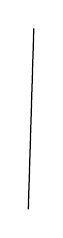
\begin{tikzpicture}[baseline=0pt,x=1cm,y=1cm]\draw[line width=.45pt] (.45,-.8)--(.52,1.5);\end{tikzpicture}}\handwritten{!}}
\uline{Lemme} 7.5. Pour tout $s\handwritten{\in}U$, il existe un élément $f\handwritten{\in}G_o$ \rlap{\begin{tikzpicture}[baseline=0pt,x=1cm,y=1cm]\draw[line width=.4pt] (-.08,-.18) .. controls (-.13,.15) and (.35,.2) .. (2.95,.34) .. controls (3.25,.36) and (3.40,.48) .. (3.28,.65);\end{tikzpicture}}\inserted{\handwritten{et $V'_o\subset\unsure{U_o|V_o}$ \unsure{stable} par $f$}} tel que le polynôme caractéristique de $f$ opérant sur \rlap{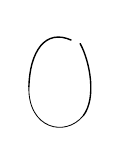
\begin{tikzpicture}[baseline=0pt,x=1cm,y=1cm]\draw[line width=.5pt] (.38,.64) .. controls (.05,.79) and (-.15,.50) .. (-.16,.04);\draw[line width=.3pt] (-.16,.04) .. controls (-.17,-.48) and (.30,-.60) .. (.53,-.32);\draw[line width=.5pt] (.53,-.32) .. controls (.70,-.1) and (.62,.36) .. (.49,.60);\end{tikzpicture}}$V_o^{\handwritten{\prime}}$ soit égal à celui de $f_s$, \deleted{P}et en particulier tel que $f\handwritten{|_{V'_o}}$ et $f_s$ aient même trace.

\uline{Lemme} 7.6. Pour tout entier $N\handwritten{\geq}0$, il existe un entier $d^{\handwritten{\prime}}_o$ \rlap{\begin{tikzpicture}[baseline=0pt,x=1cm,y=1cm]\draw[line width=.4pt] (-.03,-.28) .. controls (-.12,.19) and (.04,.33) .. (.42,.33) .. controls (.85,.33) and (1.02,.38) .. (.92,.55);\end{tikzpicture}}\inserted{\handwritten{$>0$}} tel que pour tout entier $d\handwritten{\geq}d'_o$, il existe une extension finie $k'$ de $k$ et un point $s\handwritten{\in}U_d(k')$ tel que $\operatorname{card}(Y_s)=N$. (Marche dès que $X$ est un sous-schéma fermé de $P^r_k$ de dimension $n\handwritten{\geq}1$.)

\uline{Démonstration de} 7.6. \rlap{\begin{tikzpicture}[baseline=0pt,x=1cm,y=1cm]\draw[line width=.4pt] (-.06,-.17) .. controls (-.25,.10) and (.20,.19) .. (2.7,.32) .. controls (3.09,.35) and (3.21,.48) .. (3.22,.70);\end{tikzpicture}}\inserted{\handwritten{On \unsure{peut supposer} $X$ réduit.}} Soit $r$ la \rlap{\begin{tikzpicture}[baseline=0pt,x=1cm,y=1cm]\draw[line width=.4pt] (-.05,-.2) .. controls (-.13,.13) and (.20,.24) .. (1.98,.23) .. controls (2.35,.23) and (2.52,.29) .. (2.40,.44);\end{tikzpicture}}\inserted{somme des} degrés des composantes irréductibles réduites de $X$ qui sont de\deleted{d} dimension $n$, et soit $d_1$ un entier tel que
\[
N\handwritten{\geq}rd_1^n\,.
\]
Quitte à passer à une extension finie de $k$, on peut supposer \deleted{que chaque composante irréductible $X_{\unsure{1|i}}$ de $X$ \inserted{est géom. irréductible et} contient un point rationnel sur $k$ qui $\unsure{x_i|x_1}$ n'appartient à aucun et que} les composantes irréductibles $X_i$ de $X$ géométriquement irréductibles, que tout $X_i$ contient un $x_i\handwritten{\in}X_i(k)$, et qu'il existe $n$ formes $\handwritten{\phi}_o,\,.\,.,\,\handwritten{\phi}_{n-1}$ de degré $d_1$ sur $P^r_k$,
% archive sheet number: 23
